\documentclass{article}
\usepackage[most]{tcolorbox}
\usepackage{amsmath}
\usepackage{enumitem}  
\usepackage{cmbright}
\usepackage{graphicx}



\newtcolorbox{questionbox}{
  colback=white,
  colframe=black,
  fonttitle=\bfseries,
  coltitle=black,
  boxrule=0.6pt,
  arc=2mm,
  left=2mm,
  right=2mm,
  top=1mm,
  bottom=1mm,
  enhanced,
  sharp corners=southwest,
  title=Question,
}

\begin{document}

\begin{questionbox}
\textit{It is given that four consecutive terms of a sequence are 50, 45, \(x\) and \(y\).}

\begin{enumerate}[label=(\alph*)]
    \item \textit{State the value of}
    \[
    y - x \quad \textit{if the sequence is an arithmetic progression.}
    \]

    \item \textit{$\frac{y}{x}$ if the sequence is a geometric progression.}
\end{enumerate}
\end{questionbox}

\begin{questionbox}
\textit{Diagram 1 shows two straight lines.}

\begin{center}
  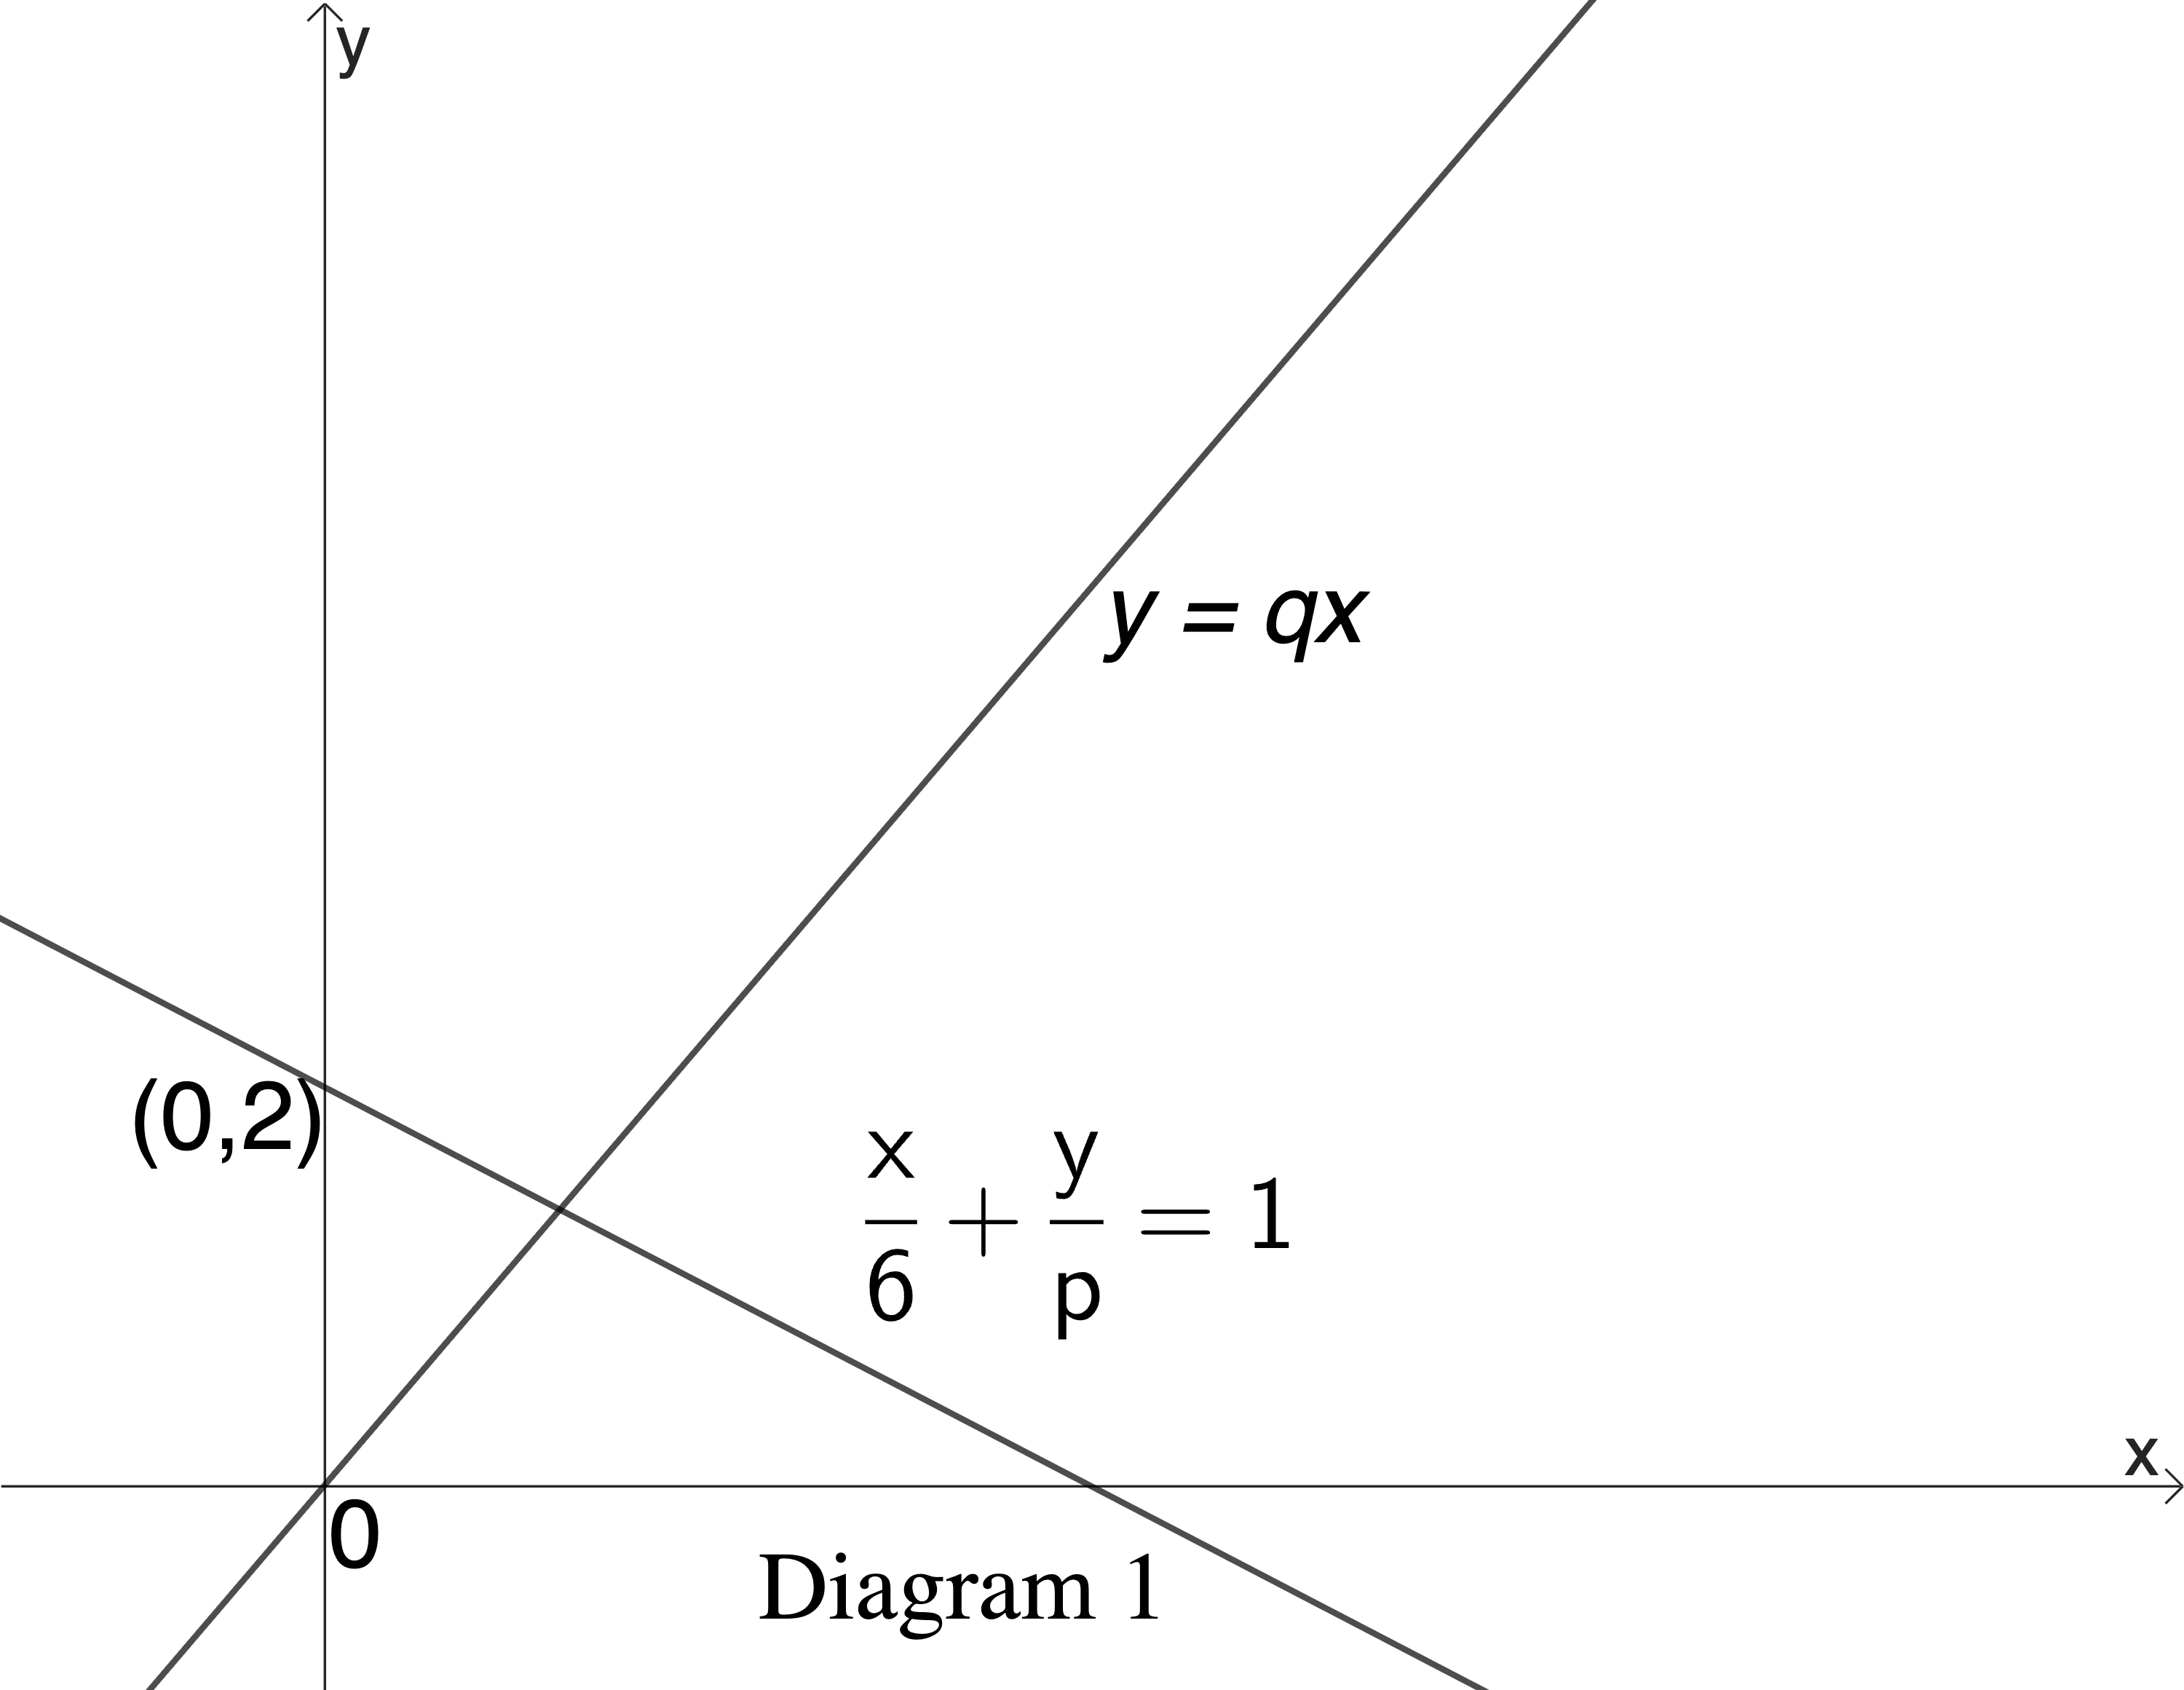
\includegraphics[width=0.5\textwidth]{png/Q2.png}
\end{center}

\vspace{0.5cm}

\textit{Find the value of q.}

\end{questionbox}

\begin{questionbox}
\textit{Diagram 2 shows two straight lines, $L_1$ and $L_2$, drawn based on 5 plotted points on a plane $\frac{1}{y}$ against $x^2$.}

\begin{center}
  \includegraphics[width=0.5\textwidth]{png/Q3.png}
\end{center}

\vspace{0.5cm}

\begin{enumerate}[label=(\alph*)]
    \item \textit{Which straight line is a suitable line of best fit? Give a reason for your answer.}

    \item \textit{Given that (10,9) lies on the line of best fit, express y in terms of x.}
\end{enumerate}

\end{questionbox}

\end{document}

